\documentclass[11pt, twocolumn]{article}
\usepackage{titlesec}
\usepackage{tikz}
\usepackage{booktabs}
\usepackage{adjustbox} 
\usepackage{enumitem}
\usepackage{multirow}
\usepackage{bbding,enumitem}
\usepackage{authblk}
\usepackage{fancyhdr}
\usepackage{amsmath}
\usepackage{subcaption}
\usepackage[table]{xcolor}
\setcounter{secnumdepth}{3} % for adjusting padding
\pagestyle{fancy}
\newcommand{\blueoval}{%
    \begin{tikzpicture}[remember picture, overlay]
    \shade[shading=axis, left color=blue, right color=white] (current page.north west) -- (3,0) arc (0:180:4cm) -- cycle;
    \end{tikzpicture}%
}

\newcommand{\coloredfooter}{%
    \begin{tikzpicture}[remember picture, overlay]
    \shade[shading=axis, left color=teal, right color=white] (current page.south east) -- (-1,-2) arc (0:80:2cm) -- cycle;
    \end{tikzpicture}%
}

\fancyhf{} % Clear default header and footer
\fancyhead[L]{ \leftmark}
% Display section title in the left header
\fancyhead[R]{\thepage} % Display page number in the right header
\definecolor{mypink3}{cmyk}{0, 0.7808, 0.4429, 0.1412}

\makeatletter
\renewcommand{\maketitle}{\bgroup\setlength{\parindent}{0pt}
\begin{flushleft}
  \textbf{\@title}

  \@author
\end{flushleft}\egroup
}
\makeatother

\title{\Huge \color{mypink3}{ROV Document}  \vspace{0.5cm}}
\author{\Large E-JUST Robotics Club \normalsize \hspace{0.5cm} }

\setlength{\parindent}{0pt}
\date{\today}

\usepackage[showframe=false, margin=.75in]{geometry}

\usepackage{abstract}
\renewcommand{\abstractname}{}    % clear the title
\renewcommand{\absnamepos}{empty} % originally center

\usepackage{lipsum}

\usepackage{afterpage}

\renewenvironment{abstract}
 {\small
  \begin{center}
  \bfseries \abstractname\vspace{-.5em}\vspace{0pt}
  \end{center}
  \list{}{%
    \setlength{\leftmargin}{10mm}% <---------- Change margin here
    \setlength{\rightmargin}{\leftmargin}%
  }%
  \item\relax}
 {\endlist}

\usepackage[utf8]{inputenc}

%\usepackage{graphicx}
\usepackage{wrapfig}
\usepackage[lofdepth,lotdepth]{subfig}
\usepackage{booktabs}

\usepackage{rotating}

\usepackage{caption}
%\usepackage{subcaption}

%\usepackage[ngerman]{babel}

\usepackage{csquotes}

\setlength{\marginparwidth}{2cm} % Set marginparwidth to avoid todonotes issues
\usepackage{todonotes}

\usepackage{stfloats}

\usepackage[T1]{fontenc}
\usepackage{textcomp}
\usepackage{times}

\usepackage{framed} %um Boxen zu machen

\usepackage[citestyle=authoryear,
			bibstyle=authoryear,
			language=auto,
			url=false,
			backend=bibtex,
			doi=false,
			isbn=false]{biblatex}
	\renewbibmacro*{volume+number+eid}{%
  \printfield{volume}%
%  \setunit*{\adddot}% DELETED
  \setunit*{\addnbspace}% NEW (optional); there's also \addnbthinspace
  \printfield{number}%
  \setunit{\addcomma\space}%
  \printfield{eid}}
\DeclareFieldFormat[article]{number}{\mkbibparens{#1}}

\usepackage{setspace}
\onehalfspacing

\setlength{\columnsep}{0.8cm}

\setlength{\parskip}{0em}

\usepackage{color}
\definecolor{black}{gray}{0} % 10% gray

\usepackage[colorlinks=true,linkcolor=black,citecolor=black]{hyperref}

\usepackage{tabularx}
\newcolumntype{s}{>{\hsize=.5\hsize}X}

\usepackage{ntheorem}
\newtheorem*{TRQ}{Research Question}

\newtheorem{Hyp}{Hypothesis} 

\usepackage{graphicx}
\usepackage{fancyhdr}
\usepackage{lipsum}
\usepackage{geometry}
\usepackage{changepage} % To adjust page margins locally
\usepackage{afterpage}

% Apply the custom header and footer to all pages
\fancyfoot[L]{\hspace*{-1.9cm}{
\includegraphics[width=\paperwidth,height=1.9cm]{Images/Footer.png}}} % Footer

\pagestyle{fancy}
\makeatletter
\providecommand{\sf@counterlist}{} % Define sf@counterlist to avoid undefined control sequence
\makeatother

\usepackage{titlesec}

\titlespacing*{\subsection}{0pt}{5pt}{5pt}
\titlespacing*{\subsubsection}{0pt}{5pt}{5pt}

\setcounter{secnumdepth}{4}
\renewcommand\theparagraph{\thesubsubsection.\arabic{paragraph}}

\usepackage{tabularray}
\DefTblrTemplate{firsthead,middlehead,lasthead}{default}{}
\DefTblrTemplate{firstfoot}{default}{
  \UseTblrTemplate{contfoot}{default}
  \UseTblrTemplate{caption}{default}
}
\DefTblrTemplate{middlefoot}{default}{
  \UseTblrTemplate{contfoot}{default}
  \UseTblrTemplate{capcont}{default}
}
\DefTblrTemplate{lastfoot}{default}{
  \UseTblrTemplate{note}{default}
  \UseTblrTemplate{remark}{default}
  \UseTblrTemplate{capcont}{default}
}
\DefTblrTemplate{contfoot-text}{default}{Continue on the next column}
\DefTblrTemplate{capcont}{default}{\UseTblrTemplate{caption}{default}}
\UseTblrLibrary{booktabs}
\captionsetup{skip=3pt}
\SetTblrInner{rowsep=0pt, stretch=0.9}
\setlength{\headheight}{13.6pt}
\addtolength{\topmargin}{-1.6pt}
\setlength{\footskip}{58.2pt}

\begin{document}

\twocolumn

Fat Man float is inspired by the NSF-funded GO-BGC Project, which aims to build a global network of profiling floats to monitor ocean health. Similarly, our float is designed to perform multiple vertical profiles, diving from the surface to a depth of 2.5 meters, then returning to the surface. It records and transmits data, simulating real-world environmental monitoring devices.

\section{Mechanical Design}

The main float body (Figure \ref{fig:float}) is constructed from a transparent acrylic cylinder measuring 40 cm in length, 12 cm in outer diameter, and 3 mm in wall thickness. Acrylic was chosen for its ability to withstand hydrostatic pressure at a depth of 2.5 meters (approximately 25 kPa), its transparency which allows for visual inspection and early error detection, and its relatively low density of 1.19 g/cm³, offering better buoyancy characteristics compared to heavier materials like PVC or HDPE. Its specifications provide sufficient water displacement, maximizing buoyancy according to Archimedes' principle (Equation \ref{eq:archimedes})

\begin{equation}
\label{eq:archimedes}
    F_B = \rho_{\text{water}} \cdot g \cdot V_{\text{disp}}
\end{equation}

An HDPE disk, a material with a density close to water, is positioned to divide the cylinder into two sections. The upper section houses the electrical components, while the lower section serves as a water chamber for density control. The disk features grooves to mount O-rings, ensuring secure isolation between the two sections. Additionally, chemical sealing agents such as epoxy are used to reinforce the isolation. The suction system uses two peristaltic pumps (Figure \ref{fig:pump}) for suction and ejection, operating at a flow rate of 60 ml/min, allowing the 700 ml chamber to be filled or emptied in approximately six minutes per operation. These pumps function by compressing a flexible tube with rotating rollers, generating a wave-like motion that pushes fluid through the tube, allowing precise flow control. To prevent leakage, the inlet and outlet hoses pass through PG-9 glands using 8 mm pneumatic hose. 

\begin{wrapfigure}{r}{0.4\columnwidth}
  \centering
  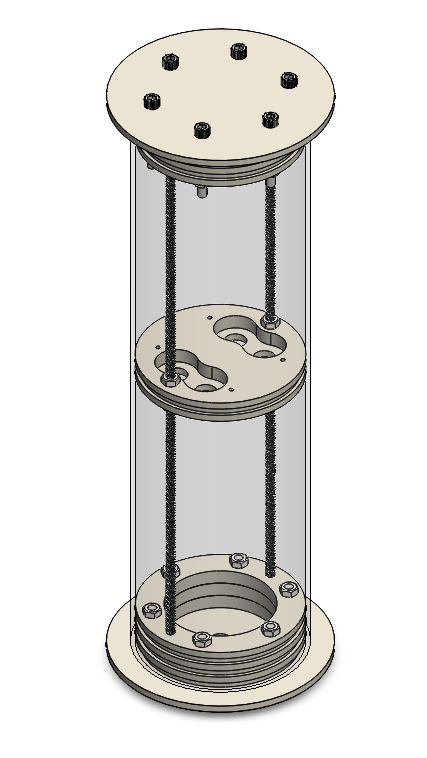
\includegraphics[width=0.39\columnwidth]{Images/Float.png}
  \caption{Illustrates the float mechanism, including 6mm lead screws, HDPE disk, and fastening nuts.}
  \label{fig:float}
\end{wrapfigure}

The float is sealed at both ends using custom end caps, each consisting of four stacked layers of HDPE. The outermost layer is 5 mm thick and exposed to water, while the remaining three layers are 10 mm thick and feature grooves designed to accommodate three O-rings for secure sealing. These layers are fastened together using bolts and nuts to ensure structural integrity and leak-proof performance. The end caps are friction-fit into the housing and are not secured with other fastening methods.

\begin{figure}[h]
  \centering
  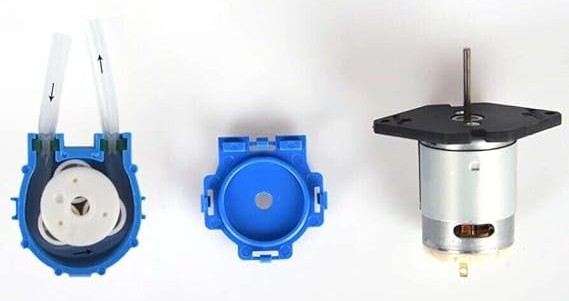
\includegraphics[width=\columnwidth]{Images/peristaltic pump.jpg}
  \caption{Illustrates the peristaltic pump inner parts and mechanism.}
  \label{fig:pump}
\end{figure}

\section{Electrical and Communication Systems}
\end{document}